\documentclass[12pt,a4paper,oneside]{ctexart}
\title{\textbf{Practice5 Report}}
\author{Name:Xu Ziyang 22320607}
\date{2023/11/8 YY/MM/DD}
\usepackage{graphicx}
\usepackage{float}
\usepackage{color}
\usepackage{amsmath}
\ctexset{abstractname=Abstract}
\begin{document}
\maketitle
\begin{abstract}
    In task1, we consider if the system state-controllable, output controllable and observable.
    In task2, we consider if the system can reach 
    $\begin{bmatrix}
        0\\
        0
    \end{bmatrix}$
    from 
    $\begin{bmatrix}
        1\\
        3
    \end{bmatrix}$ in 1 second and construct the system in simulink.
\end{abstract}
\newpage
Declare:$$k=7$$
All System:
$$\dot{\vec{x}} = A\vec{x} + B\vec{u}(t)$$
$$\vec{y} = C\vec{x} + D\vec{u}(t)$$
    \section{Task1}
        \subsection{System1}
        Declare:
            $$
            A=\begin{bmatrix}
                2-k&1\\
                0&3
            \end{bmatrix}
            $$
            $$
            B=\begin{bmatrix}
                -1\\
                2+k
            \end{bmatrix}
            $$
            $$
            C=\begin{bmatrix}
                1&0
            \end{bmatrix}
            $$
            $$
            D=0
            $$
            \subsubsection{Question1:State Controllability}
                Caculate $Q_C$.
                $$Q_C = \begin{bmatrix}
                    B&AB
                \end{bmatrix} = \begin{bmatrix}
                    -1&14\\
                    9&-27
                \end{bmatrix}$$
                $$Rank(Q_c)=2=Rank(A)$$
                So the system is controllable.

            \subsubsection{Question2:Output Controllability}
                Caculate $Q_{CO}$.
                $$Q_{CO} = \begin{bmatrix}
                    CB&CAB&D
                \end{bmatrix} = \begin{bmatrix}
                    -1&14&0
                \end{bmatrix}$$
                $$Rank(Q_{CO})=1=Rank(C)$$
                So the system is output controllable.
                
            \subsubsection{Question3:Observability}
                Caculate $Q_{O}$.
                $$Q_{O} = \begin{bmatrix}
                    C\\
                    CA
                \end{bmatrix} = \begin{bmatrix}
                    1&0\\
                    -5&1
                \end{bmatrix}$$
                $$Rank(Q_{O})=2=Rank(A)$$
                So the system is output observable.

        \subsection{System2}
        Declare:
            $$
            A=\begin{bmatrix}
                0&1+k\\
                2&0
            \end{bmatrix}
            $$
            $$
            B=\begin{bmatrix}
                0\\
                1
            \end{bmatrix}
            $$
            $$
            C=\begin{bmatrix}
                1&-1
            \end{bmatrix}
            $$
            $$
            D=0
            $$
            \subsubsection{Question1:State Controllability}
                Caculate $Q_C$.
                $$Q_C = \begin{bmatrix}
                    B&AB
                \end{bmatrix} = \begin{bmatrix}
                    0&8\\
                    1&0
                \end{bmatrix}$$
                $$Rank(Q_c)=2=Rank(A)$$
                So the system is controllable.

            \subsubsection{Question2:Output Controllability}
                Caculate $Q_{CO}$.
                $$Q_{CO} = \begin{bmatrix}
                    CB&CAB&D
                \end{bmatrix} = \begin{bmatrix}
                    -1&8&0
                \end{bmatrix}$$
                $$Rank(Q_{CO})=1=Rank(C)$$
                So the system is output controllable.
                
            \subsubsection{Question3:Observability}
                Caculate $Q_{O}$.
                $$Q_{O} = \begin{bmatrix}
                    C\\
                    CA
                \end{bmatrix} = \begin{bmatrix}
                    1&-1\\
                    -2&8
                \end{bmatrix}$$
                $$Rank(Q_{O})=2=Rank(A)$$
                So the system is output observable.

        \subsection{System3}
        Declare:
            $$
            A=\begin{bmatrix}
                -2&1\\
                1+k&3
            \end{bmatrix}
            $$
            $$
            B=\begin{bmatrix}
                0&1\\
                -2&1
            \end{bmatrix}
            $$
            $$
            C=\begin{bmatrix}
                0&1
            \end{bmatrix}
            $$
            $$
            D=0
            $$
            \subsubsection{Question1:State Controllability}
                Caculate $Q_C$.
                $$Q_C = \begin{bmatrix}
                    B&AB
                \end{bmatrix} = \begin{bmatrix}
                    0&1&-2&-1\\
                    -2&1&-6&11
                \end{bmatrix}$$
                $$Rank(Q_c)=2=Rank(A)$$
                So the system is controllable.

            \subsubsection{Question2:Output Controllability}
                Caculate $Q_{CO}$.
                $$Q_{CO} = \begin{bmatrix}
                    CB&CAB&D
                \end{bmatrix} = \begin{bmatrix}
                    -2&1&-6&11&0
                \end{bmatrix}$$
                $$Rank(Q_{CO})=1=Rank(C)$$
                So the system is output controllable.
                
            \subsubsection{Question3:Observability}
                Caculate $Q_{O}$.
                $$Q_{O} = \begin{bmatrix}
                    C\\
                    CA
                \end{bmatrix} = \begin{bmatrix}
                    0&1\\
                    8&3
                \end{bmatrix}$$
                $$Rank(Q_{O})=2=Rank(A)$$
                So the system is output observable.

        \subsection{System4}
        Declare:
            $$
            A=\begin{bmatrix}
                2&1\\
                0&k
            \end{bmatrix}
            $$
            $$
            B=\begin{bmatrix}
                1\\
                2
            \end{bmatrix}
            $$
            $$
            C=\begin{bmatrix}
                1&-2\\
                2&1
            \end{bmatrix}
            $$
            $$
            D=0
            $$
            \subsubsection{Question1:State Controllability}
                Caculate $Q_C$.
                $$Q_C = \begin{bmatrix}
                    B&AB
                \end{bmatrix} = \begin{bmatrix}
                    1&4\\
                    2&14
                \end{bmatrix}$$
                $$Rank(Q_c)=2=Rank(A)$$
                So the system is controllable.

            \subsubsection{Question2:Output Controllability}
                Caculate $Q_{CO}$.
                $$Q_{CO} = \begin{bmatrix}
                    CB&CAB&D
                \end{bmatrix} = \begin{bmatrix}
                    -3&-24&0\\
                    4&22&0
                \end{bmatrix}$$
                $$Rank(Q_{CO})=2=Rank(C)$$
                So the system is output controllable.
                
            \subsubsection{Question3:Observability}
                Caculate $Q_{O}$.
                $$Q_{O} = \begin{bmatrix}
                    C\\
                    CA
                \end{bmatrix} = \begin{bmatrix}
                    1&-2&2&-13\\
                    2&1&4&9
                \end{bmatrix}$$
                $$Rank(Q_{O})=2=Rank(A)$$
                So the system is output observable.
            \subsection{Wolfram Codes}
            \begin{figure}[p]
                \centering
                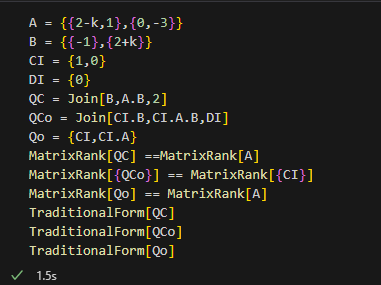
\includegraphics[height = 0.2\textheight]{../T1S1.PNG}
                \caption{System1}
                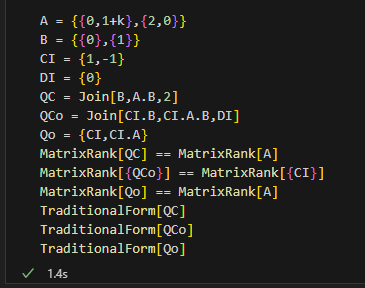
\includegraphics[height = 0.2\textheight]{../T1S2.PNG}
                \caption{System2}
                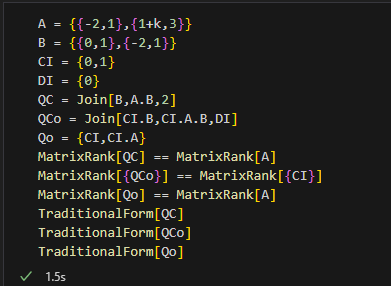
\includegraphics[height = 0.2\textheight]{../T1S3.PNG}
                \caption{System3}
                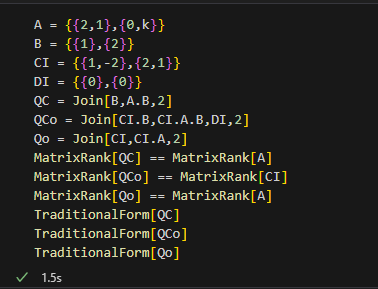
\includegraphics[height = 0.2\textheight]{../T1S4.PNG}
                \caption{System4}
            \end{figure}

            \newpage
    \section{Task2}
        \subsection{Is reachable?}
        I will directly show the code:
        \begin{figure}[H]
            \centering
            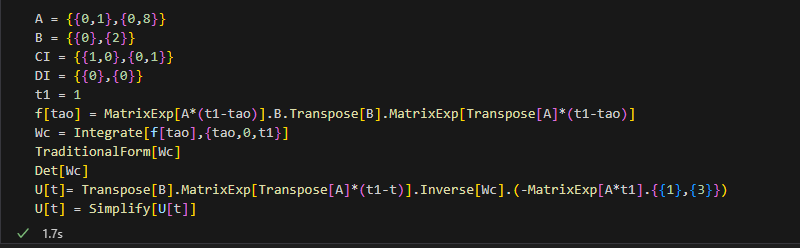
\includegraphics[width = 0.8\linewidth]{../T2.PNG}
            \caption{Code}
            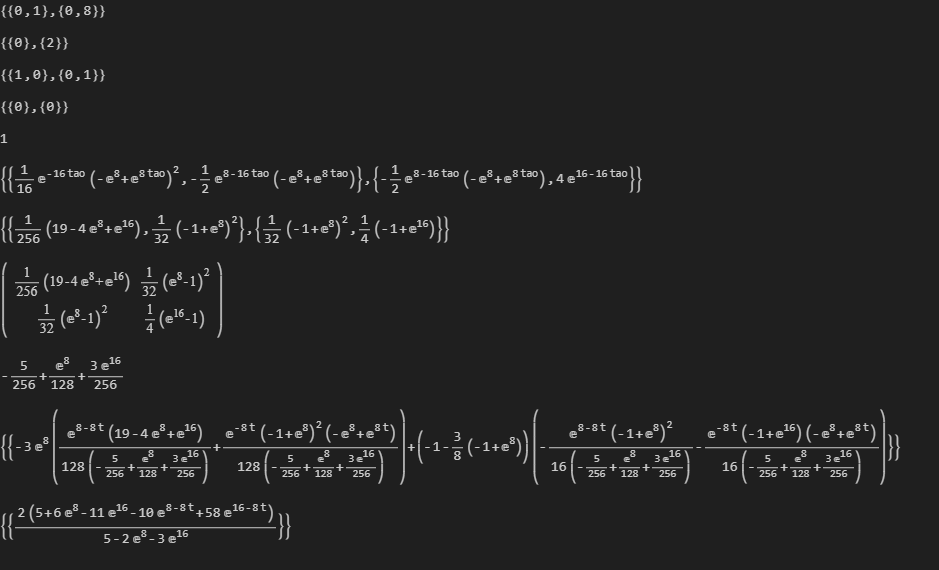
\includegraphics[width = 0.8\linewidth]{../T2A.PNG}
            \caption{Answer}
        \end{figure}
        Note $det(W_c)$ is not 0, so it is reachable.
        \newpage
        \subsection{Model}
        \begin{figure}[H]
            \centering
            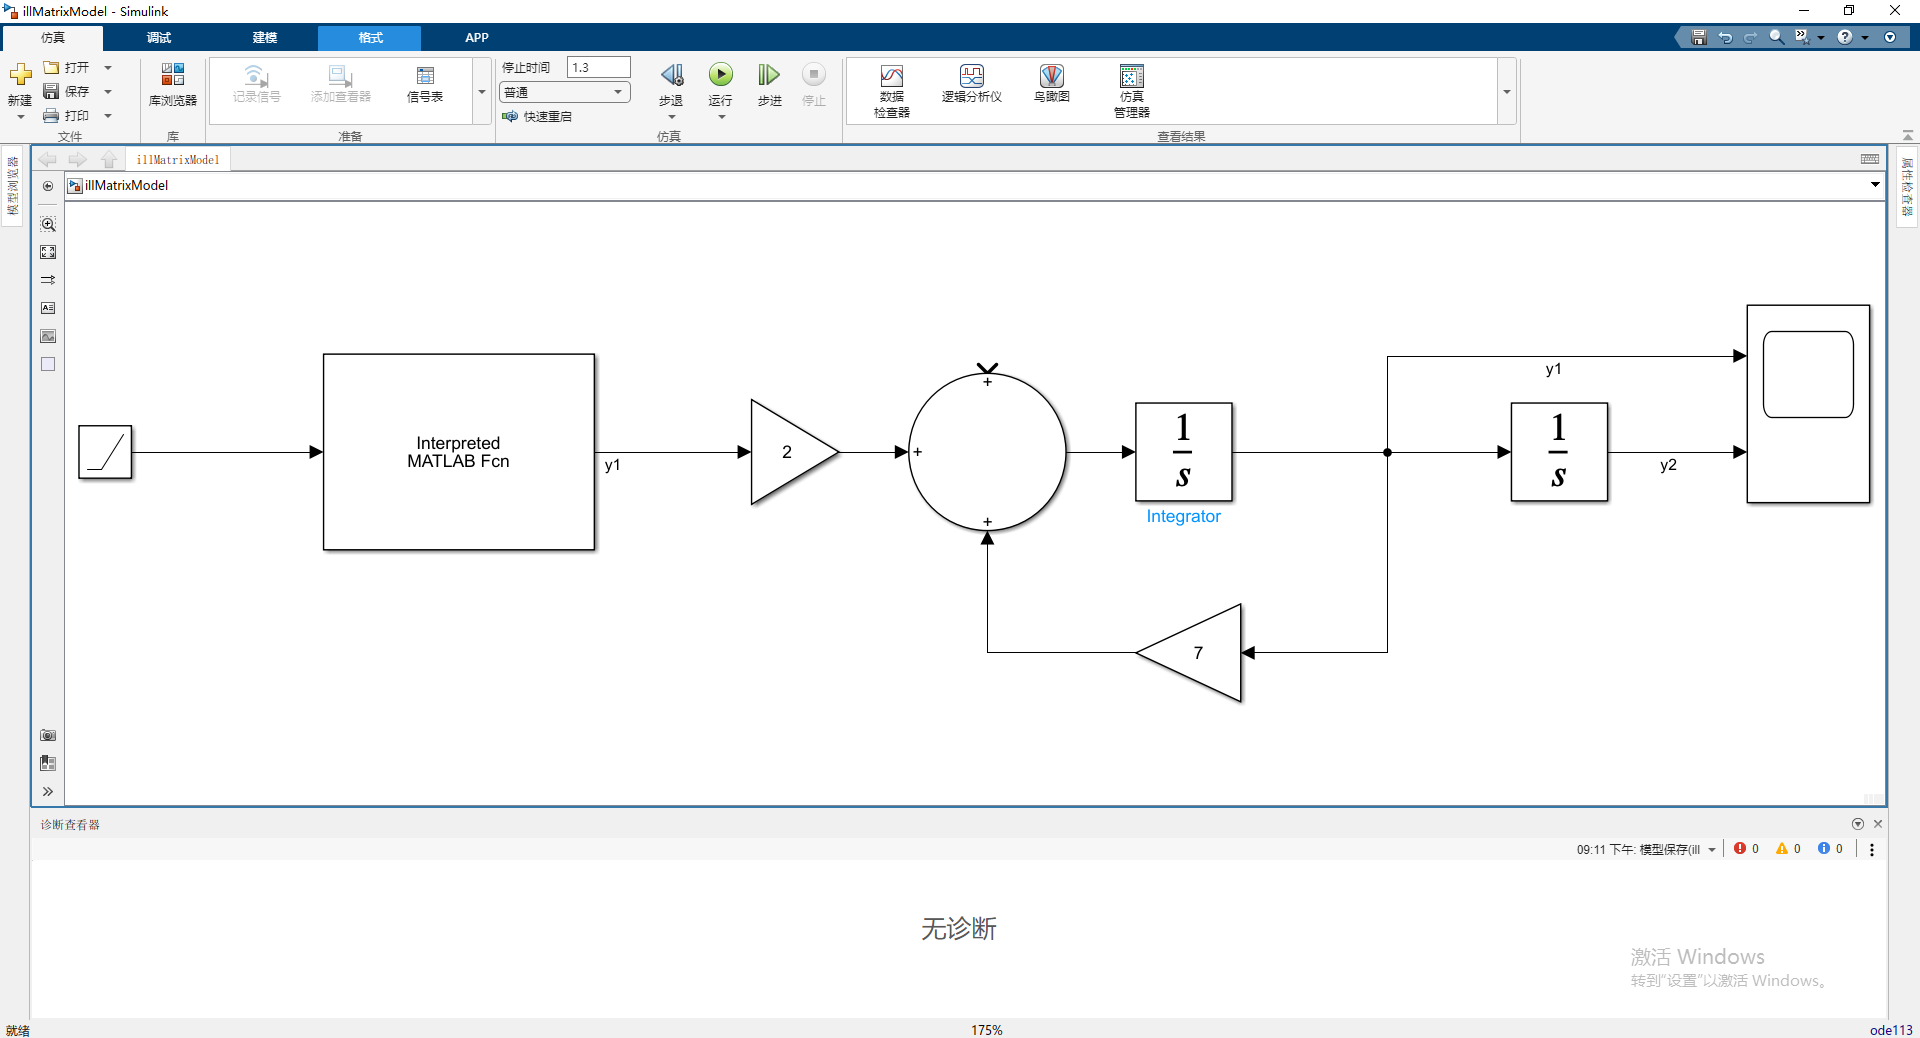
\includegraphics[width = 0.8\linewidth]{../model.PNG}
            \caption{Model}
            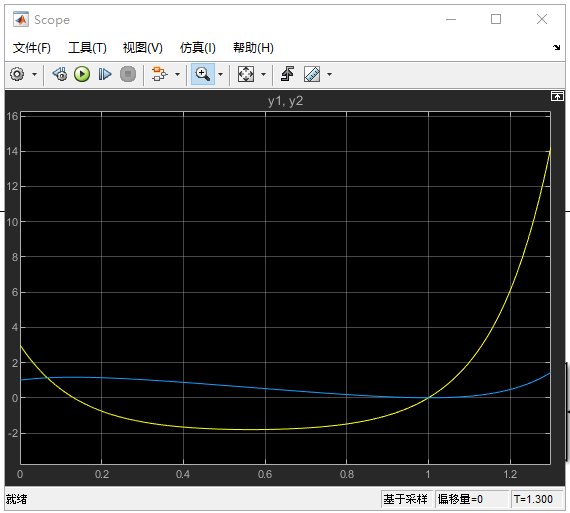
\includegraphics[width = 0.8\linewidth]{../shot.PNG}
            \caption{Figure of $y_1,y_2$}
        \end{figure}
\end{document}